% vim:spell:spelllang=en
\chapter{Register Allocation\Author{F. Bouchez, S. Hack}}
\label{chap:register-allocation}

{

%% Local macros for personal use
\newcount\todocount \todocount=0
\def\todo#1{\global\advance\todocount by 1 {\color{blue} {\bf TODO:} #1}}
\newlinechar=`\^^J
\def\endofchapter{\ifnum\todocount>0\immediate\write16{^^JLaTeX Warning: There 
was still TODO macros: \the\todocount.^^J}\fi}


\def\
\def\ac#1{#1}
\def\dom{\preceq}
\def\ssa{SSA\xspace}
\def\maxlive{\ensuremath{\mathrm{Maxlive}}\xspace}
\def\irc{Iterated Register Coalescing\xspace}

\graphicspath{{register_allocation/}{part4/register_allocation/}}

% \chapterauthor{Bouchez, Hack}

Register allocation maps the variables of a program to 
physical memory locations. The compiler determines the location for each variable and each program point.
Ideally, as many operations as possible draw their operands from processor registers without loading them from memory before. 
Due to the huge latency of the memory hierarchy (even loading from L1 cache takes 3--10 times longer than accessing a register), register allocation is one of the most important optimizations in a compiler. 

However, there is only a small number of registers available in a CPU (usual values range from~8 to~128).
Hence, the task of register allocation is not only assigning the variables to registers but also to figure out when which variables is stored to and loaded from memory (spilling).
Furthermore, register allocation also has to deal with removing spurious copy operations (copy coalescing) inserted by several phases in the compilation process before and allocation restrictions that the instruction set architecture and the runtime system imposes (register targeting).


\section{Introduction}

{\sl
\begin{itemize}
  \item based on graph coloring, linear scan
  \item spilling \& coloring are dependent
  \item heuristics are used to find a working solution
  \item avoiding spills is more important than coalescing
  \item Fab: It is important to outline that with decoupled reg-alloc, spilling and coloring become much simpler and more efficient.
\end{itemize}
}

Register allocation is usually performed per procedure.
A liveness analysis determines for each variable the program points where the variable is live.
A variable is live at a program point if there exists a path in procedure on which the variable will be used later on and is not overwritten before that use.
Hence, storage needs to be allocated for that variable; ideally a register.
The set of all program points where a variable is live is called the \emph{live range} of the variable.
The resource conflict of two variables is called \emph{interference} and is usually defined via liveness:
Two variables interfere if (and only if) there exists a program point where they a simultaneously live\footnote{
This definition of interference by liveness is an overapproximation.
There are refined definitions that create less interferences.
However, in this chapter we will restrict ourselves to this definition.
}.
The number of live variables at a program point is called the \emph{register pressure} at that program point. 
The maximum register pressure over all program points in a procedure is called the register pressure of that procedure or \maxlive.

It is helpful to think of interference as an undirected \emph{interference graph:}
The variables of the program are its nodes.
To nodes are connected if they interfere.
The set of variables live at some program point build a \emph{clique} in this graph:
Every variable in this set interferes with the other in the set, hence their nodes are all mutually connected.
The size of the largest clique in the interference graph is called its \emph{clique number} $\omega$.
A \emph{coloring} of this graph with~$k$ colors corresponds to a valid register allocation with~$k$ registers.
Hence, we will use the terms register and color in the following text.
A $k$-coloring is a mapping from the graph's nodes to the first~$k$ natural numbers (called colors) such that two neighboring nodes have different colors.
The smallest~$k$ for which a coloring exists is called the graph's~\emph{chromatic number} $\chi$.
Of course $\chi\ge\omega$ holds for every graph, because the nodes in a clique must all have different colors.

Chaitin~\cite{chaitin:1981:register} showed that for every undirected graph, there is a program that has this graph as its interference graph.
From the NP-completeness of graph coloring then follows the NP-completeness of register allocation.
Hence, determining the chromatic number of the interference graph is not possible in polynomial time unless P=NP.

This the major nuisance of classical register allocation:
The compiler cannot efficiently determine how many registers are needed.
Startling here is that one apparently might need more registers than \maxlive.
\maxlive certainly is a lower bound on the chromatic number, but the chromatic number might be greater. 
This means that although at every program point there are no more than \maxlive variables live at the same time, we still might need $>\maxlive$ registers for a correct register allocation.
This seems unintuitive at first sight but is caused by control-flow merges, as can be seen in Figure~\ref{fig:ra:exprg}.

\begin{figure}[htbp]
	\begin{center}
		\subfigure[Example program and live ranges of its variables]{ 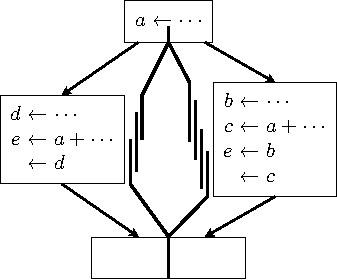
\includegraphics{figures/prog_lr.pdf} }
		\qquad
		\subfigure[Interference graph]{ 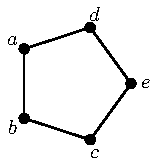
\includegraphics[scale=1.1]{figures/prog_ig.pdf} }
	\end{center}
	\caption{Example program and its interference graph}
	\label{fig:ra:exprg}
\end{figure}

In that example, the register pressure is at most~2 at every program point.
However, the interference graph cannot be colored with~2 colors. 
Its chromatic number is~3.
The inequality between \maxlive and the chromatic number is caused by the cycle in the interference graph\footnote{In theory, the gap between the chromatic number and \maxlive can even be arbitrarily large. This can be shown using by applying Chaitin's proof of the NP-completeness of register allocation to Mycielski graphs.}.

This situation changes if we permit \emph{live-range splitting.}
That is inserting a copy (move) instruction at a program point that creates a new variable and thus allows the old variable's value to change its register. 
Assume we allowed the value of~$e$ to change its register at the end of the left block by splitting~$e$'s live range into two parts (cf.~the SSA version of the program shown in Figure~\ref{fig:ra:exprgssa}).
Then, the cycle in the interference graph breaks and its chromatic number equals \maxlive.

% \begin{figure}[htbp]
% 	\begin{center}
% 		\subfigure[Example program with live range of~$e$ split]{ 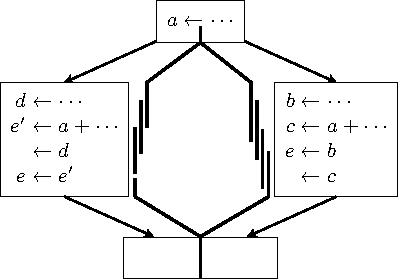
\includegraphics{figures/prog_split_lr.pdf} }
% 		\qquad
% 		\subfigure[Interference graph]{ 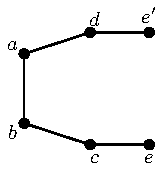
\includegraphics[scale=1.1]{figures/prog_split_ig.pdf} }
% 	\end{center}
% 	\caption{Example Program with spit live range and its interference graph}
% 	\label{fig:ra:exprgsplit}
% \end{figure}

In an extreme setting, one could split the live ranges of all variables after every instruction.
Then, the interference graph degenerate into several disconnected components and its chromatic number drops to \maxlive.
Of course such an extreme live-range splitting introduces a lot of shuffle code which degrades the runtime of the compiled program.
This interplay between live-range splitting and colorability is the key issue in register allocation.

\subsection{Non-SSA Register Allocators}
As finding a valid $k$-coloring is NP-complete, assigning registers is performed by some heuristic algorithm.
If that algorithm fails to find a free register for a variable, spilling is activated to free one.
The problem here is that the spilling decision is made to revive the coloring heuristic not because the variable is actually a good candidate for spilling. 
Even more, we might even spill a variable because the heuristic is ``not good enough'' not because we are out of registers.

At the same time, classical techniques perform copy coalescing (i.e.~undoing live-range splitting) during coloring.
However, if done aggressively, coalescing can make the graph harder to color or make the heuristic fail and thus introduce spills.
This is of course unacceptable because we never want to access memory in favor of an eliminated copy.
Thus, existing techniques often apply \emph{conservative} coalescing approaches which do not increase the chromatic number of the graph.

\subsection{Why SSA helps}

The live ranges in an SSA-form program all have a certain property:
SSA requires that all uses of a variable are dominated by its definition.
Hence, the whole live range is dominated by the variable's definition.
Dominance, however, induces a tree on the control flow graph.
Thus, the live ranges of SSA variables are all tree-shaped~\cite{bouchez,brisk:2006:poly,HGG:2006:RA_SSA}.
They can branch downwards the dominance tree but have a single root: the program point of the variable's definition.
Hence a situation like in Figure~\ref{fig:ra:exprg} where the live range of~$e$ has two ``roots'' can no longer occur.
The live range of~$e$ is split by a \phifun in the corresponding SSA program.
The result variable of that \phifun constitutes a new live range.
The register allocator now has more freedom:
The two operands of the \phifun and its result variable can be assigned to different registers.

\begin{figure}[htbp]
	\begin{center}
		\subfigure[example program in SSA]{ 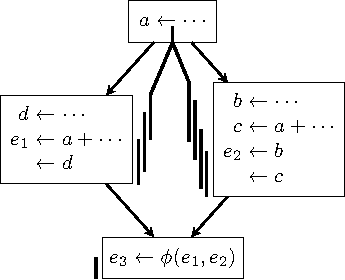
\includegraphics{figures/prog_ssa_lr.pdf} }
		\qquad
		\subfigure[Interference graph]{ 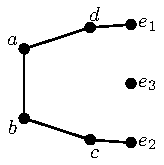
\includegraphics[scale=1.1]{figures/prog_ssa_ig.pdf} }
	\end{center}
	\caption{SSA version of the example program}
	\label{fig:ra:exprgssa}
\end{figure}

This special structure of the live ranges leads to a special class of interference graphs:
Gavril~\cite{gavril:1974:trees} showed, that the intersection graphs of subtrees are the \emph{chordal graphs}.
Chordal graphs can be optimally colored in linear a time with respect to the number of edges in the graph.
Furthermore, they are \emph{perfect} which means that for every subgraph, the clique number equals the chromatic number. 
This is a very important property for register allocation because it means that \maxlive equals the chromatic number of the graph\footnote{
This also implies that chordal graphs do not have ``holes'' like the interference graph in Figure~\ref{fig:ra:exprg}.
Every cycle is spanned by \emph{chords.}
}:
Even more, one can show~\cite{bouchez,HGG:2006:RA_SSA} that for every clique in the interference graph, there is one program point where all the variables of that clique are live.
This decouples spilling from coloring:
First, we lower the register pressure to~$k$ everywhere in the program.
Then, we can color the interference graph with~$k$ colors in polynomial time.

\subsection{Maxlive and colorability of graphs}

{\sl
\begin{itemize}
  \item definition of Maxlive
  \item show that Maxlive is the minimum number of colors required
  \item scan of the dominance tree sufficient to know Maxlive: pseudo-code
  \item Fab: MAXLIVE minimum if interference graph==intersection graph. Clearly we do not want to go into such details but be careful to use precise and correct terms.
\end{itemize}
}
    
The register pressure at a program point is the number of variables alive at 
this point.\footnote{Considering all simultaneously alive variables interfere.}
The greatest register pressure over all a program is called \maxlive, 
since it is the maximum number of simultaneously alive variables. Obviously, 
spilling is mandatory if \maxlive is strictly greater than $R$, the number of 
registers.
Under SSA, the good news is that this is the only case where spilling is 
required, i.e., if \maxlive $\leq R$, there is no need for spilling. Indeed, 
\maxlive is the coloring number of the chordal interference graph of the 
program (\todo{ref to chapter 2?}). So, we can devise a polynomial test to know 
whether spilling is necessary or not by computing \maxlive. This can be done by 
checking on every program point the number of variables that are alive. If 
liveness information is available on the whole program, the order does not 
matter. However, in the case of SSA, this is not required as \maxlive can 
easily be computed without liveness information by performing a scan of the 
dominance tree, starting from the root. We only need to know which uses are 
``last-uses.'' The pseudo-code is given on Figure~\ref{code:compute-maxlive}.
\todo{check \maxlive scan needs last uses}.


\begin{figure}[ht]
  \begin{verbatim}
  function compute-branch (p, live)
    live <- live - { uses in p that are last uses }
    live <- live + { definitions of p }
    maxlive <- max( maxlive, #live )
    foreach child c of p
      compute-branch (c, live)

  function compute-maxlive
    maxlive <- 0
    compute-branch (root, {})
  \end{verbatim}
  \caption{Pseudo-code for \maxlive}
  \label{code:compute-maxlive}
\end{figure}




\section{The problem of spilling}
\subsection{Lowering Maxlive}

{\sl
\begin{itemize}
  \item The min number of colors is Maxlive. Variables must be stored in memory 
    to lower the register pressure at points where it is $>R$.
  \item Whenever, Maxlive $\leq R$, we know for sure that spilling more in 
    unnecessary.
  \item Fab: if MAXLIVE$\leq R$ spilling is unecessary under some conditions (we color SSA code, going out of SSA code might require some additionnal spilling. Also without naming constraints). So again be careful about what you say. I think that the idea is to have a register allocator under SSA as simple as possible with a very simple modeling and nice properties. Then we cope with real world issues during the colored-SSA destruction.
\end{itemize}
}

Usually, there are too many variables in a program and \maxlive is greater than 
$R$. In that case, we need to lower the register pressure at program points 
where it exceeds $R$ by spilling, i.e., storing variables in memory instead of 
registers. Whenever we reach a point where \maxlive $\leq R$, it will be 
possible to color all SSA variables with the $R$ registers. For now, the 
difficulty lies in choosing which variables to spill, and where to spill them. 
Indeed, a careful choice will lead to performance, while making bad decisions 
can lead to big slowdowns. As accesses to variables in memory require more time 
that accesses to registers, it is for instance better to avoid spilling 
variables used inside frequently executed code regions like loops.

\todo{spilling while keeping SSA property}


\subsection{Spilling is a difficult problem}

The problem of spilling is a difficult one in the literature, even under one of 
its simpler forms, the spill everywhere problem, where spilled variables stay 
so on their entire live-range~\cite{todo}. This spilling is advocated on the 
first graph-coloring algorithms~\cite{Chaitin81} and even in subsequent 
algorithms~\cite{IRC} because it fits better the graph-coloring representation. 
In these schemes, this amounts to removing nodes from a non $R$-colorable graph 
until it becomes $R$-colorable. Although this node deletion problem is known to 
be NP-complete, this allows the writing of simple heuristics based on the 
number of neighbours in the graph and a cost attached to nodes representing the 
overhead incurred in case they were to be spilled. An added problem is the fact 
that, for many architectures like RISC, spilled variables cannot be accessed 
directly from memory but must instead by copied back to the registers, when 
they are used, or which must be in a register when defined, just before being 
copied to memory. This creates new variables with very short live-ranges at the 
definition and use points, which must be accounted for register allocation. 
This explains why algorithms such as \irc must rebuild the interference graph 
after a phase of spilling and start again, until no more spilling is required.


The actual spilling problem is even more difficult, as variables do not have to 
be spilled on their entire live-range.
% borrowed from sebastian's CC'09 paper
Consider a loop with excessive register pressure and a variable that is defined 
before the loop and used afterwards. Ideally, a compiler would store (spill) 
the variable in front of the loop and load (reload) the variable after the 
loop. If the variable was reloaded inside the loop, the reload would be 
executed in each loop iteration. Another example is a variable that is used in 
a loop but has already been spilled before the loop. Reloading this variable 
directly before its use in the loop will cause memory traffic in each loop 
iteration. Thus, it is preferable to put the reload in front of the loop.
% end of borrowing
This poses a new problem on top of choosing which variables to spill: now we 
need also to choose where to spill them, i.e., where to put {\tt load} and {\tt 
store} instructions. This more general problem where the goal is to minimize 
the overhead of these added instructions is called the load-store optimization 
problem and is known to be NP-complete, even for a 
basic-block~\cite{Liberatore00}.  


\subsection{SSA does not help for spilling}
{\sl
\begin{itemize}
  \item easy spill method: spill everywhere
  \item SSA split points are good for coloring, but not really for spilling 
    (see article spill everywhere under SSA)
  \item other split points to avoid spill everywhere are probably better
  \item Fab: if you need an example to illustrate that SSA does not really help 
    in practice for spilling ask Quentin. It does help a little bit (dynamic 
    programming possible for spill everywhere with few registers; further first 
    can be generalized). But what you want to point it here is the fact that 
    the disadvantages seem more important than advantages.
  \item Fab: the LCTES spill everywhere article does not discuss practical issues (such as the fact that it might insert a load or a store inside a loop...). It is more algorithmical issues.
  \item Seb: Want do we want to say here?
  	  I think the title of the section is too negative. 
  	  Perhaps we should merge the section with the last.
  	  I think it would be good to first talk about different definitions for spilling,
  	  then give an overview over your results (LCTES paper).
\end{itemize}
}

For the spilling problem, the SSA is not really of much help. Over a blind 
spill everywhere algorithm on the initial program, it has however the slight 
advantage of allowing the spilling of SSA variables, i.e., sub-variables of the 
initial variables. One major disadvantage is the added complexity when spilling
variables defined in \phifuns \todo{explain the problem if not all args are 
spilled, or if spilled in $\neq$ locations}.
\todo{Seb: complexity? perhaps slight complications :)}

{\sl Examples by Quentin}
\begin{minipage}{.45\textwidth}
\begin{verbatim}
CSSA :
   a =
   b =
 /       \
c= a   d = b
 \       /
 e = phi(c,d)
 = e
\end{verbatim}
\end{minipage}
\begin{minipage}{.45\textwidth}
After spilling spill :
\begin{verbatim}
   a =
   b =
 /          \
c= a     d = b
C=st c  D = st d
 \          /
 E = phi(C,D)
 e = ld E
 = e
\end{verbatim}
\end{minipage}
In that case, memory locations C, D and E can be the same. But this does not 
mean that placement of {\tt store} instruction is the best one.

\begin{minipage}{.45\textwidth}
\begin{verbatim}
SSA :
   a =
   b =
 /         \
 \         /
 e = phi(a,b)
 = e
\end{verbatim}
\end{minipage}
\begin{minipage}{.45\textwidth}
Spill supposing {\tt store}s are after definition
\begin{verbatim}
   a =
   A = st a
   b =
   B = st b
 /         \
 \ <--     / <--
 E = phi(A,B)
 e = ld E
 = e
\end{verbatim}
\end{minipage}

On the two edges pointed by arrows (or on the preceding basic block if they are 
not critical), additional memory transactions must reconcile the values:
\begin{verbatim}
tmp = ld X
Y = st tmp
\end{verbatim}

This can induce more spill, unforeseen.
Without SSA, this problem does not exist: for instance, with spill everywhere, 
the same memory slot is affected to all definitions of the same variable so no 
post-treatment is required as it is under SSA.



\subsection{Spilling under SSA}
Still, we give a possibility to perform spilling under SSA
\begin{itemize}
  \item Hack's algorithm: simplified version?
  \item \`a la Belady following dominance tree?

  \item Fab: The last Algorithm from Sebastian is Belady like. So yes try to simplify it, provide the pseudo code and give the intuitions on how the full version improves it.
  \item Seb: I think it's ok to briefly outline the approaches that are out there and refer to the papers.

\end{itemize}
\todo{Ask Sebastian to do it.}


\cite{Braun09:spilling-ssa}\todo{file braun09cc.pdf in biblio}


\section{Coloring and coalescing}
\subsection{Chordal property for coloring}

{\sl
\begin{itemize}
  \item two simplicial nodes
  \item color in the reverse order of simplification
  \item one such order considers subtrees from the root of the tree
  \item no need to construct interference graph
  \item Fab: make it as more intuitive as possible. Avoid as much as possible 
    chordal stuffs which are useless. Greedy coloring and its relationship with 
    the subtree representation is important on the other hand. See with Philip 
    to avoid redundancies between your chapter and his (SSA properties). It is 
    important to outline here that this property that is due to decoupled+SSA 
    enables more aggressive coalescing heuristics. But also simpler 
    (tree-scan).
\end{itemize}
}

\subsubsection{The greedy coloring scheme.}

In traditional graph coloring register allocation algorithms, the assignment is 
done by coloring the interference graph using a greedy heuristic. This greedy 
scheme is based on the observation that, given $R$ registers (colors), if a 
node in the graph has at most $R-1$ neighbours, there will always be one color 
available for this node for any coloring of the remaining of the graph. Hence 
this node can be \emph{simplified}, i.e., removed from the graph and placed on 
a stack. This process can be iterated with the remaining nodes, and if the 
graph becomes empty, we know it is possible to color the graph with $R$ colors. 
Such a coloring can be obtained by assigning colors to nodes in the reverse 
order of their simplification, i.e., by popping nodes from the stack and, since 
they have at least $R-1$ colored neighbours assigning them one available color. 
We call this algorithm the \emph{greedy coloring scheme}. Whenever this scheme 
gets stuck, i.e., if all remaining nodes have degree at least $R$, we do not 
know whether the graph is $R$-colorable or not since it is just a heuristic.


\subsubsection{Greedy-$k$-colorable graphs.}

An interesting fact is that the success or failure of this greedy scheme is 
independent of the order of simplification. In other words, if the greedy 
scheme fails at some point, there is no simplification order that could 
simplify entirely the graph. This is because the remaining nodes have degree 
greater than~$R$ at all time and there is no way to reduce their degree than 
simplifying one of them, which is impossible. The side effect is that the 
greedy scheme defines a class of graphs that we call the 
\emph{greedy-$k$-colorable} graphs. These are the graphs $k$-colorable using 
the greedy scheme. The pseudo-code for testing if a graph is 
greedy-$k$-colorable is given on Figure~\ref{code:is-k-greedy}.



\begin{comment}
\begin{function}[h]
\captionlabel{\labelkgreedy}{Is\_kGreedy}{($G$)}
\KwData{Undirected graph $G=(V,E)$; $\forall v\in V$, degree[$v$] = \#neighbors 
of $v$ in $G$, $k$ number of colors}
% \lForEach{$v\in V$}{set degree[$v$] to degree of $v$ in $G$ \;}
stack = $\emptyset$ ;
$\mbox{worklist} = \{ v \in V \mid \mbox{degree[$v$]} < k\}$ \;
\While{$\mbox{worklist} \neq \emptyset$}{
  \KwLet $v \in \mbox{worklist}$ \;
  \ForEach{$w$ neighbor of $v$}{
     degree[$w$] \<- degree[w]-1 \;
     \lIf{$\mbox{degree[$w$]} = k-1$}{worklist \<- $\mbox{worklist} \cup \{w\}$}
  }
  push $v$ on stack ;
  worklist \<- $\mbox{worklist} \setminus \{v\}$  \tcc*{Remove $v$ from  $G$}
}
\lIf{$V = \emptyset$}{\Return{\KwTrue}}
\lElse{\Return{\KwFalse}}
\end{function} 
\end{comment} 

\begin{figure}
\begin{verbatim}
Function Is_kGreedy(G)
  Data: Undirected graph G = (V, E);
  ∀v ∈ V, degree[v] = #neighbors of v in G,
  k number of colors
stack = {} ; worklist = {v ∈ V | degree[v] < k} ;
while worklist != {} do
  let v in worklist ;
  foreach w neighbor of v do
    degree[w] = degree[w]-1 ;
    if degree[w] = k - 1 then worklist = worklist U {w}
  push v on stack ; worklist = worklist \ {v} ; /* Remove v from G */
if V = {} then return TRUE else return FALSE
\end{verbatim}
\caption{Iskgreedy function}
\label{code:is-k-greedy}
\end{figure}

\subsubsection{Simplification on chordal graphs.}

Chordal graphs are easily colorable using a \emph{simplicial elimination 
scheme}. There is indeed a property that chordal graph have at least two 
simplicial vertices, i.e., nodes whose neighbours in the graph are a clique (a 
complete subgraph) \todo{check if already said in chapter 2, or cf. Appendix}.  
A simplicial elimination scheme is a particular order of simplification of 
nodes in which only simplicial nodes may be chosen. Such an order gives the 
minimum number of colors to the graph in polynomial time, but can be a bit 
tedious to obtain. In practice, in register allocation, we do not need the 
minimum number of colors, we just need that at most $R$ colors are used. Since 
enough spilling has already been done in the previous section, we know that 
\maxlive is at most $R$, hence that the interference graph is $k$-chordal with 
$k\leq R$. This means that every simplicial node in the simplicial elimination 
scheme has a degree at most $k-1$ in the remaining graph, hence any simplicial 
elimination order is also a valid simplification order for a 
greedy-$k$-coloring. Hence a $k$-chordal graph is also greedy-$k$-colorable, 
hence greedy-$R$-colorable and any simplification scheme for $R$ registers will 
manage to color it with at most $R$ colors.


This means we do not need a fancy coloring algorithm tuned for chordal graphs, 
the original simplification scheme of Chaitin et al.\ does the job, without any 
modification. Following a call to Is\_k\_Greedy, it is possible to re-use the 
stack to assign the colors by making a call to Assign\_colors, 
Figure~\ref{code:assign-color}. Among the good things, this also means that 
existing register allocators can be easily modified to handle SSA code and that 
register allocation can benefit from powerful coalescing strategies such as 
aggressive or conservative ones. Moreover, the fact that register allocation 
can be decoupled into a phase of spilling first and then a phase of 
coloring/coalescing allows the writing of more involved coalescing \todo{cite 
examples}.


\begin{figure}
\begin{verbatim}
Function Assign_colors(G)
  available = new array of size R and values True
  while stack != {} do
    v = pop stack ;
    for each neighbour w in G
      available[color(w)] = False
    col = 0;
    for each color c from 1 to R
      if available[c]
        col = c
      available[c] = True /* prepare for next round */
    color(v) = col
    add v to G
\end{verbatim}
\caption{Assign\_color function}
\label{code:assign-color}
\end{figure}





\subsection{Fast tree-scan solution}
{\sl
\begin{itemize}
  \item On the dominance tree, possible to scan from top and assign colors to 
    variables as they come.
  \item Biased coloring is used to coalesce variables linked by \phifuns.
  \item see next section for more involved coalescing
  \item Fab: I think that you already talked about scan coloring. Ok to talk about biased.
  \item Fab: You can talk about biased coloring that uses the result of an aggressive coalescing (see with Quentin). It is not more complicated and it improves results.
\end{itemize}
}

One of the advantages of SSA is to make things simpler, faster, and use less 
memory. For the register assignment problem, we have seen that the existing 
greedy scheme based on simplification still works, however, this still requires 
the construction and maintaining of an interference graph, a structure judged 
to big and cumbersome to be used in JIT context, where compilation time and 
memory prints matters more. This is one of the reasons linear-scan allocators 
are being developed, even if their performance does not equal those of 
aggressive time-consuming off-line compilers. We will now present a method to 
perform fast register assignment for SSA programs which does not need more than 
the dominance tree and def-use chains.

Let us get back at the dominance tree representation, with live-ranges being 
subtrees of this tree. This representation reflects the chordal property of the 
interference graph. Consider the variables alive at a leaf of the dominance 
tree (the ``end'' of a branch), they form a clique of the graph and because of 
the dominance property, the definition of one of them, say $v$, is dominated by 
the definitions of all the others.  This variable has a ``smaller'' live-range, 
compared to the other variables, which are all already alive at its definition.  
This means that every variable interfering with $v$ also interfere with the 
other variables. In other words, all neighbours of $v$ form a clique, i.e., $v$ 
is a simplicial node in the interference graph, and it has at most $R-1$ 
neighbours.  This means that all ``leaf'' variables, i.e., the ones that have 
their definition the closest to the end of their branch in the dominance tree, 
are candidate for simplification by the greedy algorithm. Once they are 
simplified, other variables become leaf variables and the simplification 
process can continue again, until we reach the root of the dominance tree.

Following the idea of the greedy algorithm, the stack is now filled with 
variables ordered by appearance of their definition, i.e., if the definition of 
$a$ appears before the definition of $b$ on the path from the root to $b$, $a$ 
is higher in the stack, hence will be colored before $b$. In short, it is 
possible to color all subtrees of the dominance tree by starting at the root 
and scanning the dominance tree in a top-down fashion, assigning colors to 
variable as their definition is encountered. This is possible since, under SSA,  
variables are subtrees hence do not interfere if they belong to different 
branches. A pseudo-code to assign colors is given in procedure Tree\_Scan,
Figure~\ref{code:assign-tree-scan}.


\begin{figure}
  The {\tt colors} array is boolean and represent available colors.

  \begin{verbatim}
Tree_Scan(T)

  function assign_color(p,colors)
    for each v last use at p
      colors[color(c)] = True   /* colors not used anymore */

    for each v defined at p
      choose_color(v,colors)    /* choose available color */
      colors[c] = False
      color(v) = c

    for each child p' of p
      assign_color(p', colors)

  color(root(T))

  \end{verbatim}
  \caption{Tree scan coloring algorithm for SSA.}
  \label{code:assign-tree-scan}
\end{figure}


This coloring algorithm is really fast as it only needs one traversal of the 
dominance tree. Since the number of colors is fixed and small, it can be 
implemented as a bit-set so as to speed-up updates of which colors are 
available or not. The pseudo-code for function {\tt choose\_color} is 
deliberately not given yet. A very basic implementation can just scan the 
color array until it finds one that is not taken (this is assured since we are 
under SSA and spilling has already been done). We will now see why it might be 
beneficial to bias the choosing of colors so as to perform some coalescing.



\subsubsection{Biased coalescing.}

The goal of coalescing is to minimize the number of register-to-register {\tt 
move} instructions in the final code. While there may not be so many such 
``copies'' at the high-level (e.g., instruction {\tt a = b} in C), especially 
after a phase of copy propagation under SSA (\todo{See chapter X}), there can 
be much more of these after the register allocation phase. One reason is that 
it helps treating register constraints, we will explain this point in 
Section~\ref{sec:practical-regalloc}. One even more obvious and unavoidable 
reason is the presence of \phifuns due to SSA form. Indeed, remember that a 
\phifun represents in fact parallel copies on incoming edges of basic blocks. 
For instance, if the function is $a \gets \phi(b,c)$, then it means that 
instructions $a\gets b$ should be executed on the edge coming from the left, 
and $a\gets c$ on the one from the right. Suppose now that register allocation 
decided to put $a$ and $b$ in register $R_1$, but $c$ in register $R_2$, then 
the copy $a\gets b$ does not need to be executed anymore, but $a\gets c$ does 
since the value of variable $c$, will be contained in $R_2$ and needs to 
transfered to $R_1$, which means the final code will contain instruction {\tt 
mov $R_1$, $R_2$} or the like.

Obviously, it is better to assign variables linked by a \phifun, as definition 
and argument, to the same register. This concerns for instance all subscripts 
of the same variable: it is usually better to assign $a_1$, $a_2$, etc.\ to the 
same register since they come from the same variable $a$. In fact we can define 
a notion of \emph{affinity}, acting as the converse of the relation of 
interference, expressing how much two variables ``want'' to have the same 
color, i.e., share the same register. A metric can be added to this notion, 
measuring the benefit one could get if the two variables are assigned to the 
same register. Hence, for two variables $a$ and $b$, count 1 for each time they 
appear in the same copy instruction ($a\gets b$ or $b\gets a$) or \phifun 
($a\gets\phi(\ldots,b,\ldots)$ or $b\gets\phi(\ldots,a,\ldots)$). These numbers 
can of course be weighted using empirically parameters (classically, times ten 
for each level of nested loop, halved if in a conditional branch, etc.) or 
using actual execution frequencies based on profiling.


Since the number of affinities is sparse compared to the number of possible 
pairs of variables, we propose to keep for each variable a list affinities, 
where each element is a pair composed of a variable and the weight of the 
affinity with this variable. In that case, the function {\tt choose\_color} can 
be written as in Figure~\ref{code:choose-color}. This is a very simple bias, 
where at each point the color chosen is the one that maximizes, under the 
current knowledge, the coalescing for the variable being colored. It is not of 
course optimal since the general problem of coalescing is NP-complete 
(\todo{ref}), and biased algorithms are known to be easily misguided.


\begin{figure}
  The {\tt colors} array is boolean and represent available colors.

  \begin{verbatim}
global variables
  count = array of size #colors and elements 0

choose_color(v, colors)
  for each (u,w) in affinity_list(v)
    count[color(u)] += w
  max_w = -1
  col = 0
  for each color c
    if colors[c] = true /* color is not used by a neighbour of v */
      if count[c] > max_w
        col = c
        max_w = count[c]
    count[c] = 0 /* prepare array for next call to choose_color */
  \end{verbatim}
  \caption{Choosing a color with a bias for coalescing.}
  \label{code:choose-color}
\end{figure}


\subsubsection{Aggressive coalescing to improve biased coalescing.}

There is another simple and interesting idea to improve biased coalescing. We 
still consider a JIT context where compilation speed is very important.
\todo{what kind of aggressive? Ask fab\ldots}






\section{Practical and advanced discussions}
\label{sec:practical-regalloc}


\subsection{Handling registers constraints}
{\sl
\begin{itemize}
  \item ABI contraints
  \item split beforehand solution: many parallel copies, need good biased 
    coloring
  \item repair afterwards solution: biased try to give right color, else, 
    actual copies are added
  \item Fab: For the repair afterward at the time we will publish the book you 
    will be able to cite the current paper we write on tree-scan coalescing. We 
    plan to elaborate on the repairing mechanism and illustrate it in the 
    context of tree-scan.
  \item Fab: For the repair afterward you will build an interference graph with 
    negative affinity weights. Current coalescers do not handle it. A 
    workaround (but costly) for affinity adge (a,b) with weight W<0 is replace 
    it by an interference edge (a,ab) and an affinity edge (ab,b) of weight -W 
    with ab a dummy node. For iterated reg-alloc (Briggs \& George's test) you 
    can rewrite the different rules by doing as if you had such a dummy node 
    (you virtualize it). You can discuss this with Quentin. Of course the idea 
    is not to describe it here but it can be interesting to discuss a little 
    bit the implications.
\end{itemize}
}

In theory, register allocation algorithms are always nicely working with nodes 
and colors. In practice, however, not all variables or registers are 
equivalent. Depending on the architecture, some registers might be dedicated 
to perform memory operations, some instructions expects their operands to 
reside in particular registers, and in general conventions are defined to 
simplify for example the writing of libraries, by specifying how parameters to 
functions are passed and how results are returned. This adds constraints to the 
register allocation, usually by restricting the coloring possibilities of 
variables. Some examples are given in Figure~\label{fig:reg-constraints}.

\begin{figure}
  \begin{tabular}{ccc}
    Constraint  & Instruction & Effect on reg. alloc. \\
    Division in registers $R_x$ and $R_y$ & $a / b$ & $a$ in $R_x$, $b$ in $R_y$\\
    Memory load cannot use $R_z$ & $a = load(b)$ & $b$ cannot be in $R_z$\\
    Functions arguments in $R_1$, $R_2$\ldots & $a = f(b,c)$ & $b$ in $R_1$, 
    $c$ in $R_2$ \\
  \end{tabular}
  \caption{Examples of register constraints.}
  \label{fig:reg-constraints}
\end{figure}


The problem with such constraints is that they cannot be expressed directly in 
the register allocation problem. For instance, if variable $a$ and $b$ must 
absolutely reside in register $R_1$, it is not possible to pre-color them with 
color $R_1$ as the interference graph could not be chordal anymore.  
Furthermore, $a$ and $b$ maybe interfere, for instance if they are both the 
first parameter of successive function calls, it that case putting them in the 
same register without check would break the program. We propose two solutions 
to deal with this problem. The first is classic in the literature, and the 
second is newer and promising.


\subsubsection{Splitting variables to handle register constraints.}

Traditionally, variables involved in constraining operations are split before 
and after the operation. For instance, if $a$ is involved in a division on an 
x86, the instructions $a'\gets a$ and $a\gets a'$ are issued before and after 
the division so that, if $a$ is not in the right register, it can be moved in 
it for the operation. This however still poses the problem of variable $a'$ 
which still interfere with every variable alive during the division, and hence 
is part of the interference graph. Moreover, $a$ is redefined which breaks the 
SSA. A workaround solution is to split \emph{all} variables alive before and 
after the operation using a \emph{parallel copy}. New subscripted variables 
must be defined by the second split to keep the SSA property (and subsequent 
uses must be changed accordingly). The use of parallel copies assures that 
the locally created variables, with very short live-ranges (span of only one 
instruction), are completely disconnected from the interference graph. Their 
only relation with the other, ``normal'' variable are affinities that each 
variable share with the two other parts coming from the same original variable.
In that case, the danger is that many copy instructions can be added if the 
coalescing is not good enough to assign most of the created copies to the same 
register.


\subsubsection{Repairing problems afterwards.}

Another possibility is to let register allocation do its job, and then 
intervene to repair the coloring whenever it does not fit the constraints, by 
adding copies afterwards around mismatches. To minimize the number of conflicts 
on constraints, it is however important to drive the coloring so that it still 
gives the right color whenever possible. For example, if variable $a$ must 
reside in register $R_1$, it is possible to consider a clique of $R$ nodes 
otherwise disconnected from the graph, one for each register, and adding $R_1$ 
in the affinity list of $a$. On the contrary, if $a$ cannot be assigned to a 
register, say $R_2$, an affinity of \emph{negative weight} is added to the 
list, representing the added cost it will required if $a$ is still put in 
register $R_2$. Existing coalescing algorithms in the literature currently do 
not support negative weight \todo{see Fab's hack}.








\subsection{Out-of-SSA and critical edge splitting}

{\sl
\begin{itemize}
  \item \phifuns are not machine instructions, they are replaced by actual 
    copies in out-of-SSA phase
  \item in our case, colored SSA: Sreedhar not possible
  \item SSA implicitly 
    actual ``parallel copies'' are placed on edges
  \item problem with some critical edges: abnormal edges, back-edge of loop
  \item Fab: Sreedhar IS possible. It generates local variables not colored.
The point is that its coloring might be stucked (Chaitin reduction). So the possible need to split edges...
\end{itemize}
}

As mentioned previously, the \phifuns are not actual machine instructions.  
They must be removed when going ``out-of-SSA.'' In traditional translation 
out-of-SSA, this happens before register allocation, but in our case, variables 
are already allocated to memory or registers, and arguments and results of 
\phifuns are not variables anymore but registers.


If the definition and arguments 
of a \phifun have been allocated to the same register, then it can be safely 
removed. If this is not the case, however, the some {\tt move} instructions 
must be added to keep the behaviour of the program. 



\subsection{More repairing on \phifuns}
\begin{itemize}
  \item Biased coloring is fast but not very good at coalescing
  \item Basic parallel copy motion: move to next edge.
  \item More involved problem: spill variables
  \item Better solution: look at biblio (parallel copy motion)
  \item Fab: Yes make it as simple as possible. Local pcopy motion works in practice. It is useless to go further. The ultimate solution (Sreedhar based) might have been discussed in the previous section
\end{itemize}


\endofchapter
}
